% GENERATED by mb5.paper_numbers from paper/figures/figures.tex (mb5.figures)
\begin{figure*}[t]
  \centering
  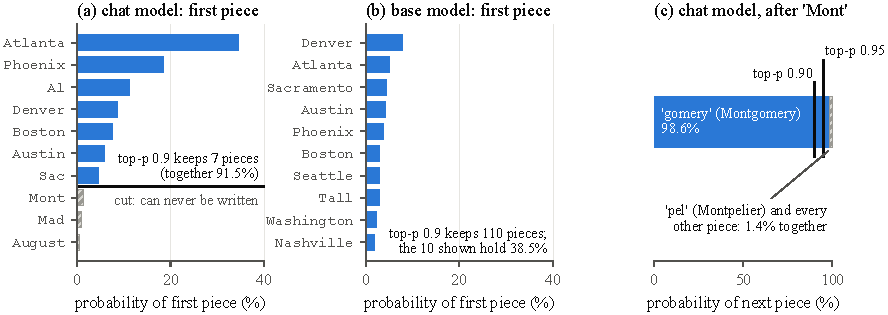
\includegraphics[width=\textwidth]{figures/fig1_mechanism.pdf}
  \caption{How a name becomes unreachable. Prompt: ``Name a capital city of a U.S. state.'' (a) The chat model's ten most likely first pieces. Top-p 0.9 keeps the 7 pieces above the line (91.5\% of the probability) and deletes the rest, so no capital starting with a deleted piece can be written. (b) The base model spreads its first step: its top piece has 7.8\% and top-p 0.9 keeps 110 pieces. (c) A name can also be cut later. After the shared piece `Mont', the chat model puts 98.6\% on `gomery' (Montgomery), so `pel' (Montpelier) is deleted even at top-p 0.95. Hatched: deleted pieces.}
  \label{fig:mechanism}
\end{figure*}
